\chapter{IMPLEMENTATION}

\section{Plugin architecture}

MeshLab loads filters as dynamic libraries discovered at startup via Qt's \texttt{QPluginLoader}. A filter plugin inherits from \texttt{FilterPlugin}, is annotated with \texttt{Q\_OBJECT} and \texttt{Q\_PLUGIN\_METADATA} so the Qt MOC can wire it up, and overrides a handful of virtual methods that report metadata, declare parameters, and execute the filter. The MeshLab UI is generated automatically from the parameter list, so the only UI code needed in the plugin is the \texttt{initParameterList} call that registers the seven user parameters with their types, defaults, and tooltips.

\begin{figure}[H]
    \centering
    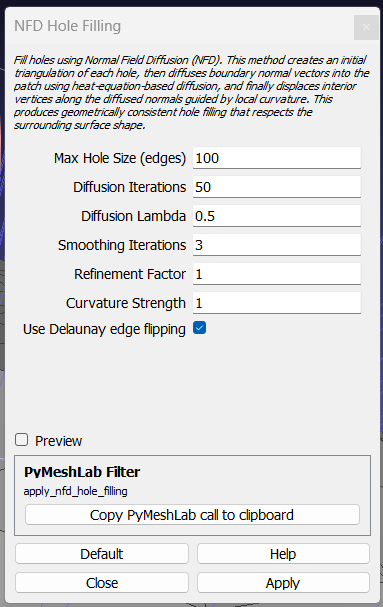
\includegraphics[width=0.5\textwidth]{figures/fig_meshlab_dialog.png}
    \caption{Filter parameter dialog generated from plugin metadata.}
    \label{fig:meshlab-dialog}
\end{figure}

The plugin is built as a CMake \texttt{MODULE} target that links against \texttt{meshlab-common}, \texttt{vcg}, and \texttt{Qt5::Core}. The output DLL goes to MeshLab's \texttt{plugins/} directory under the build tree.

\section{VCGlib usage}

VCGlib provides the mesh data structures, topology helpers, and adjacency iterators. The plugin uses:

\begin{itemize}[noitemsep]
    \item \texttt{EnableFFAdjacency} / \texttt{EnableVFAdjacency} to allocate adjacency storage on demand.
    \item \texttt{UpdateTopology::FaceFace} / \texttt{VertexFace} to populate adjacency pointers.
    \item \texttt{UpdateFlags::FaceBorderFromFF} to mark border edges, after which border tests reduce to an $O(1)$ flag query.
    \item \texttt{UpdateNormal::PerVertexNormalizedPerFace} to compute area-weighted vertex normals.
    \item \texttt{vcg::face::VFIterator} to walk the faces incident to a vertex.
    \item \texttt{vcg::tri::Allocator::AddVertices} / \texttt{AddFaces} to grow the mesh in Stage~7.
\end{itemize}

The mesh type \texttt{CMeshO} uses VCGlib's Optional Components Framework: components such as normal, colour, and adjacency are enabled per-vertex or per-face only when needed, so the storage cost matches actual usage.

\section{Eigen for the diffusion solver}

The diffusion step lives entirely in Eigen. The system matrix is built by accumulating cotangent contributions into an \texttt{Eigen::Triplet} list and committing them with \texttt{setFromTriplets}. The factorisation is one line:

\begin{lstlisting}
Eigen::SimplicialLDLT<Eigen::SparseMatrix<double>> solver;
solver.compute(A);                  // factorisation, once
for (int it = 0; it < iterations; ++it) {
    Eigen::MatrixXd rhs = ...;      // current state + boundary contribution
    normals = solver.solve(rhs);    // triangular solves, fast
}
\end{lstlisting}

\texttt{SimplicialLDLT} suits this problem: the matrix is SPD, sparse, and constant across iterations, which is exactly the factor-once / solve-many pattern the solver is built for. The boundary normals are eliminated from the unknown vector at assembly time and reappear on the right-hand side, which is the standard finite-element treatment of Dirichlet conditions.

\section{Parameters and code layout}

The seven parameters exposed to the user are summarised below. In practice, the two parameters that most often need adjustment are \texttt{CurvatureStrength} and \texttt{RefinementFactor}.

\begin{table}[H]
\centering
\caption{Plugin parameters.}
\label{tab:params}
\begin{tabularx}{\textwidth}{l l r X}
\toprule
\textbf{Parameter} & \textbf{Type} & \textbf{Default} & \textbf{Effect} \\
\midrule
\texttt{MaxHoleSize}         & int   & 100  & Skip holes longer than this. \\
\texttt{DiffusionIterations} & int   & 50   & Stage~4 iterations. \\
\texttt{DiffusionLambda}     & float & 0.5  & Stage~4 time step. \\
\texttt{SmoothingIterations} & int   & 3    & Stage~5 iterations. \\
\texttt{RefinementFactor}    & float & 1.0  & Triangle size relative to boundary edge. \\
\texttt{CurvatureStrength}   & float & 1.0  & Multiplier on cap height. \\
\texttt{UseDelaunayFlipping} & bool  & on   & Toggle Delaunay flips (off for demos). \\
\bottomrule
\end{tabularx}
\end{table}

The plugin source consists of two files: \texttt{filter\_nfd\_holefill.h} (about 70 lines, class declaration and structs) and \texttt{filter\_nfd\_holefill.cpp} (about 1\,250 lines, the full pipeline). Functions in the cpp file are laid out in pipeline order, so reading top-to-bottom follows Chapter~4. The plugin maintains no global state.

\section{Build}

The host build is MeshLab itself; the plugin is a sub-target of MeshLab's CMake project. The full build requires a one-time \texttt{cmake -G Ninja} configuration followed by \texttt{cmake --build .}\ from the MeshLab root. Incremental rebuilds of just the plugin are driven by a small batch script that calls \texttt{vcvarsall.bat x64} and rebuilds the \texttt{filter\_nfd\_holefill} target. Running MeshLab from the build tree picks up the plugin automatically.

\begin{figure}[H]
    \centering
    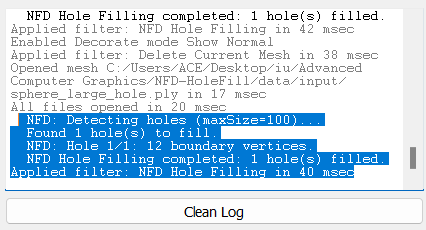
\includegraphics[width=0.85\textwidth]{figures/fig_meshlab_log.png}
    \caption{MeshLab log output after a successful filter invocation.}
    \label{fig:meshlab-log}
\end{figure}
